\documentclass[a0paper,portrait]{baposter}

\usepackage[font=small,labelfont=bf]{caption} % Required for specifying captions to tables and figures
\usepackage{booktabs} % Horizontal rules in tables
\usepackage{relsize} % Used for making text smaller in some places

\usepackage{amsmath,amsfonts,amssymb,amsthm} % Math packages
\usepackage{eqparbox}
\usepackage{easySymbols}
\usepackage{textcomp}

\graphicspath{{figures/}} % Directory in which figures are stored

 \definecolor{bordercol}{RGB}{40,40,40} % Border color of content boxes
 \definecolor{headercol1}{RGB}{186,215,230} % Background color for the header in the content boxes (left side)
 \definecolor{headercol2}{RGB}{120,120,120} % Background color for the header in the content boxes (right side)
 \definecolor{headerfontcol}{RGB}{0,0,0} % Text color for the header text in the content boxes
 \definecolor{boxcolor}{RGB}{210,235,250} % Background color for the content in the content boxes


\begin{document}

\background{ % Set the background to an image (background.pdf)
\begin{tikzpicture}[remember picture,overlay]
\draw (current page.north west)+(-2em,2em) node[anchor=north west]
{
\includegraphics[height=1.1\textheight]{background}};
\end{tikzpicture}
}

\begin{poster}{
grid=false,
borderColor=bordercol, % Border color of content boxes
headerColorOne=headercol1, % Background color for the header in the content boxes (left side)
headerColorTwo=headercol2, % Background color for the header in the content boxes (right side)
headerFontColor=headerfontcol, % Text color for the header text in the content boxes
boxColorOne=boxcolor, % Background color for the content in the content boxes
headershape=roundedright, % Specify the rounded corner in the content box headers
headerfont=\Large\sf\bf, % Font modifiers for the text in the content box headers
textborder=rectangle,
background=user,
headerborder=open, % Change to closed for a line under the content box headers
boxshade=plain
}
{
\includegraphics[scale=0.15]{logo.png}}
%
%----------------------------------------------------------------------------------------
%	TITLE AND AUTHOR NAME
%----------------------------------------------------------------------------------------
%
{ \bf  \huge {Nested Bootstrapping} \\  \it for reliable Gene Regulatory Network Inference } % Poster title
{\vspace{0.3em} \smaller Daniel Morgan$^1$ $^2$,Andreas Tj\"{a}rnberg$^3$, Torbj\"{o}rn  Nordling$^4$, Erik Sonnhammer$^1$ $^2$   \\  % Author names
% * <tn@kth.se> 2016-09-17T15:44:57.495Z:
%
% Should I not be an author too?
%
% ^ <dcolinmorgan@gmail.com> 2016-09-17T21:57:01.266Z.
  
\smaller $^1$\it {DBB, Stockholm University} \\ $^2$\it{SciLifeLab}\\ $^3$\it{Department of Physics, Chemistry and Biology / Bioinformatics, Link\"{o}ping University} \\$^4$\it {Mechanical Engineering, National Cheng Kung University} } % Author email addresses
{
\includegraphics[scale=0.4]{SciLifeLab_logo.png}} % University/lab logo

%----------------------------------------------------------------------------------------
%	INTRODUCTION
%----------------------------------------------------------------------------------------
\headerbox{Introduction}{name=introduction,column=0,row=0, span=3}{
% \vspace{0.025cm}
\begin{itemize} 
\item Common Gene Regulatory Network (GRN) inference methods, such as LASSO, do not provide information about the confidence of inferred links. We address this by extending the bootstrap method, instead overlapping the analysis in iterated runs, and applying it to three inference methods.
% * <tn@kth.se> 2016-09-17T15:49:58.986Z:
%
% > to overlap analysis of iterated run
%
% Consider rephrasing
%
% ^.
\vspace{-0.2cm}
\item Details of the shortcomings of L1-regularization methods when operating over sufficiently informative data are known. Here, all of the referenced methods perform sub-optimally in terms of Matthew's Correlation Coefficient (MCC) for low signal-to-noise ratio (SNR) data matrices, even when the data are informative enough for network inference by other metrics \cite{Tjarnberg2014}. It is thus important not only to introduce methods which are optimized for analyzing datasets of certain quality, but also to define criteria for determining which method to use to optimize analysis.
% * <tn@kth.se> 2016-09-17T15:52:47.457Z:
%
% > but also to define criteria for judging datasets to enable optimized analysis.
%
% Do you mean to define criteria for determining which method to use? If so please write it.
%
% ^.
% * <tn@kth.se> 2016-09-17T15:51:44.756Z:
%
% > sub-optimally for low signal-to-noise ratio (SNR) data matrices, even when the data are informative enough for network inference by other metrics
%
% Is the data informative enough or not? If it is then according to which measure/metric?
%
% ^.
\vspace{-0.2cm}
\item When considering which gene-gene interactions are true, we seek to differentiate spurious gene-gene interactions from those that truly exist in the system. %LASSO, Least Squares (LS) and Total Least Squares (TLS) select for highly bootstrap supported links. 
To this end we use a linear ODE model and the GeneSPIDER package to infer the regulatory network of interactions by relating the effect of single gene perturbations to the expression of the remaining unperturbed set.
\end{itemize}
% \vspace{0.0125cm}
}

%----------------------------------------------------------------------------------------
%	Materials
%----------------------------------------------------------------------------------------
\headerbox{Materials}{name=materials,column=0,below=introduction}{
\textbf{Model:} $  \mY = -\mA^{-1}\mP +\mA^{-1}\mF + \mE$\\
\textbf{Y}: expression data\\
\textbf{A}: network\\
\textbf{P}: perturbation matrix\\
\textbf{E}: input noise estimate\\
\textbf{F}: output noise estimate\\
\textbf{Gene perturbation dataset:}
\begin{enumerate}
\item 40 genes, 3 biological replicates, 2 technical replicates
\item siRNA knockdowns\\
% * <tn@kth.se> 2016-09-17T15:55:46.076Z:
%
% Are these used in some way, i.e. the negative controls, that is essential for the presentation here? If not leave them out.
%
% ^ <dcolinmorgan@gmail.com> 2016-09-17T22:03:22.674Z:
%
% just a queue to wet lab work that might engage DBB people
%
% ^.
Our experimental setup allowed us to see the individual, although not necessarily direct, effects of single gene perturbations on the remaining gene array; we also measured mixed effects by perturbing pairs of genes.\\
\textbf{$\Rightarrow$ 40 single gene perturbations}\\
\textbf{$\Rightarrow$ 40 double gene perturbations}\\
\textbf{$\Rightarrow$ qRTPCR of all 40 genes}


% \textbf{$\Rightarrow$ RNA spike:} normalize overall gene expression via standard not associated with MYC

% \textbf{$\Rightarrow$ Positive Control:} reference control (no siRNA treatment, GAPDH, ATCB standards)

% \textbf{$\Rightarrow$ Negative Control:} non-amplifiable control (no Taq, PCR should NOT work)

\item  gene fold change + variance of expression measurement
% * <tn@kth.se> 2016-09-17T15:57:52.061Z:
%
% You should separate the captions for fig 3 and fig 4. I have never seen to figure captions written together like this before.
%
% ^ <dcolinmorgan@gmail.com> 2016-09-17T22:05:15.383Z:
%
% I agree but for space consideration it will make the poster too long so I can up with this solution
%
% ^.
% * <tn@kth.se> 2016-09-17T15:56:58.480Z:
%
% > ene fold change + 
%
% Why not make a small figure? It would make it so much more clear how the experiments were done.
%
% ^.
\end{enumerate}

}

%----------------------------------------------------------------------------------------
%	WORKFLOW
%----------------------------------------------------------------------------------------
\headerbox{NestBoot Workflow}{name=workflow,span=2,column=1,below=introduction}{ 
\vspace{-0.2cm}
\begin{center}
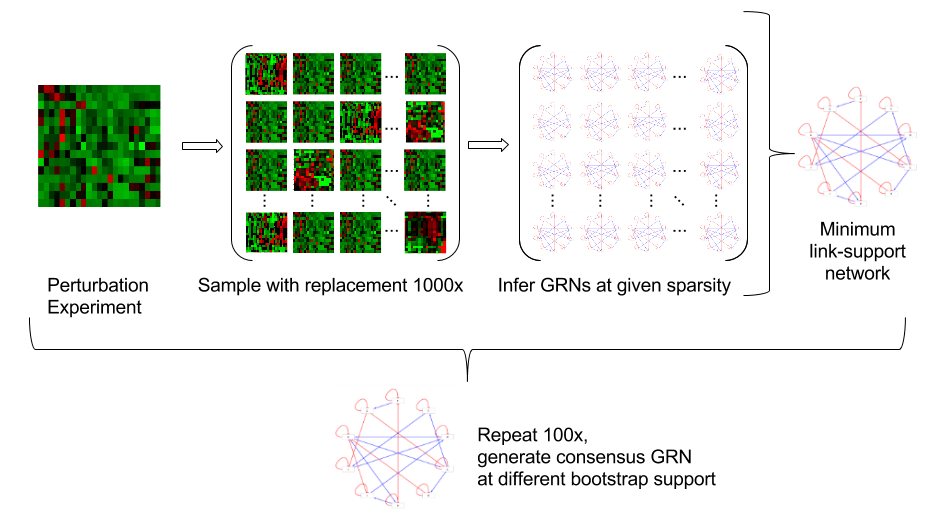
\includegraphics[width=1\linewidth]{NestBoot_method.png}
\end{center}
\vspace{-0.5cm}
}
%----------------------------------------------------------------------------------------
%	INFERENCE
%----------------------------------------------------------------------------------------
\headerbox{Inference Methods}{name=inference,span=1,column=0,below=materials}{ % To reduce this block to 1 column width, remove 'span=2'

% \begin{center}
% \resizebox{0.9\textwidth}{!}{\begin{minipage}{\textwidth}
% \begin{tabular}{l l l l}
% \toprule
% \textbf{Method} & \textbf{Equation} \\
% \midrule
% LS & $\{ \hat{A}_{ls},\Delta _{ls} \}: = \arg \min\limits_{X,\Delta A} ||\Delta A||_F$ \\ 
% & $\hat{A}_{OLS} = {{(X^TX)}^{-1} X^Ty}$ \\ \\
% TLS & $\svd[X \; Y] = U S V^T$ \\
%   & $\hat{A}_{TLS} = -\frac{VXY}{VYY}$\\ \\
% LASSO & $\min \frac{1}{2m} \norm{\mA_i\mY^T+\mP^T_i}^2_F + \zeta \norm{\mA}_1$ \\ \\
% RNI & $ \sum\limits_{j \epsilon \nu} \tilde{\phi}_j \alpha_{ij}= \tilde{\mathcal{E}}_i $\\ \\
% ARACNe & $I({x_i},{y_i})=\frac{1}{M}$$\sum\limits_{i}\log\frac{f(x_i,y_i)}{f(x_i)f(y_i)}$\\

% \bottomrule
\end{tabular}
\end{minipage}}
\end{center}
\begin{center} \vspace{.05cm}
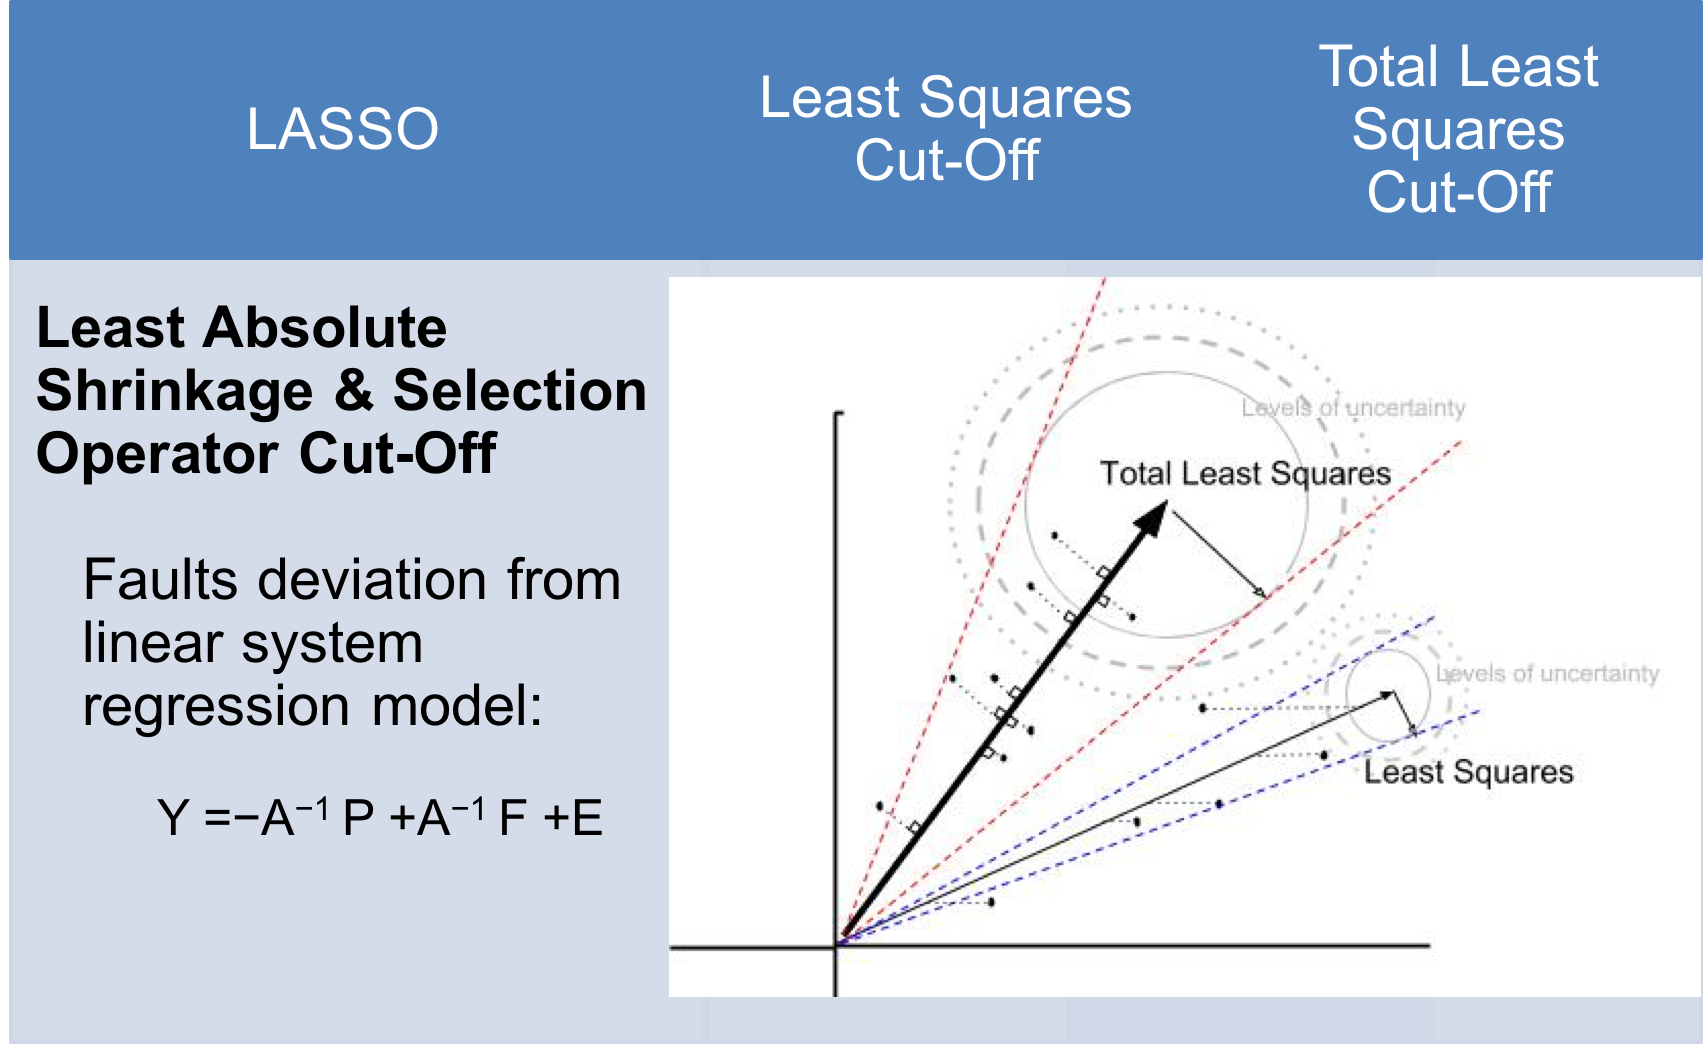
\includegraphics[width=.8\linewidth]{methods.png}
% \hspace{.5cm}\vspace{.1cm}
% 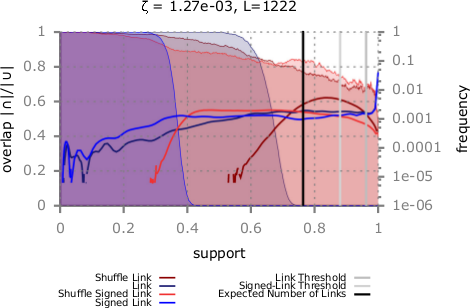
\includegraphics[width=.4\linewidth]{1222.png}
\end{center}
\vspace{-.3cm}
\small \textit{\textbf{Figure 1.} Depiction of differing link inclusion methods, including LASSO, LSCO and TLSCO; the later two differ in their consideration of correction in one and two dimensions, respectively.}} 
(left) and \textbf{Figure 4.} Here we can expect that the random data has more links at 100\% support. This sparsity level gives 756 links and the same when shuffled gives an estimated 900. Bootstrap frequency for 100 bootstrap runs with 1000 bootstraps for both real and shuffled perturbation data (right). Shaded areas show network overlap and vertical lines show lasso sparsity (black) and first crossing of shuffle over non shuffled frequency (grey).}}
% * <tn@kth.se> 2016-09-17T16:00:45.422Z:
%
% > Inference Methods (left) 
%
% Why do you include our uncertainty figure and why don't you explain it? 
%
% ^.
% * <tn@kth.se> 2016-09-17T16:00:00.442Z:
%
% > Bootstrap frequency for 100 bootstrap runs with 1000 bootstraps for both real and shuffled perturbation data (right). Shaded areas show network overlap and vertical lines show lasso sparsity (black) and first crossing of shuffle over non shuffled
%
% Please start with the result shown in the figure. Then explain the figure.
%
% ^.
% \vspace{0.15cm}



% %----------------------------------------------------------------------------------------
% %	INFERENCE PERFORMANCE
% %----------------------------------------------------------------------------------------
% \headerbox{Inference Performance}{name=inferencePerf,span=2,column=1,below=introduction}{
% \begin{center}
% % 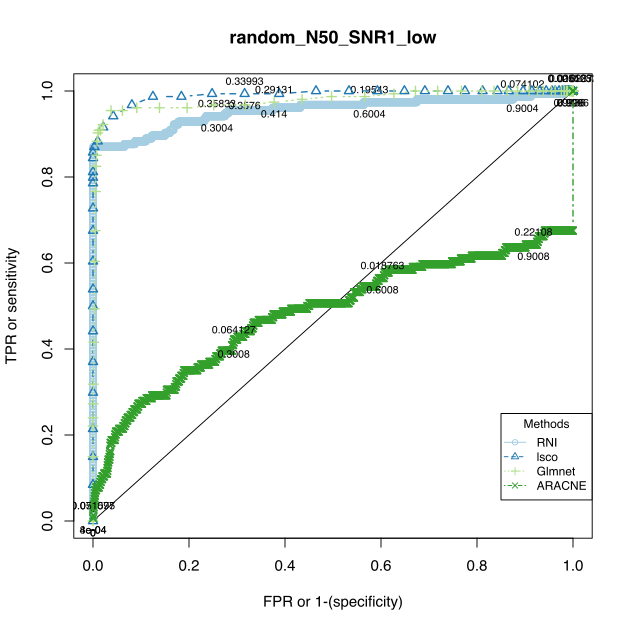
\includegraphics[width=.3\linewidth]{random_N50_SNR1_low.png}
% 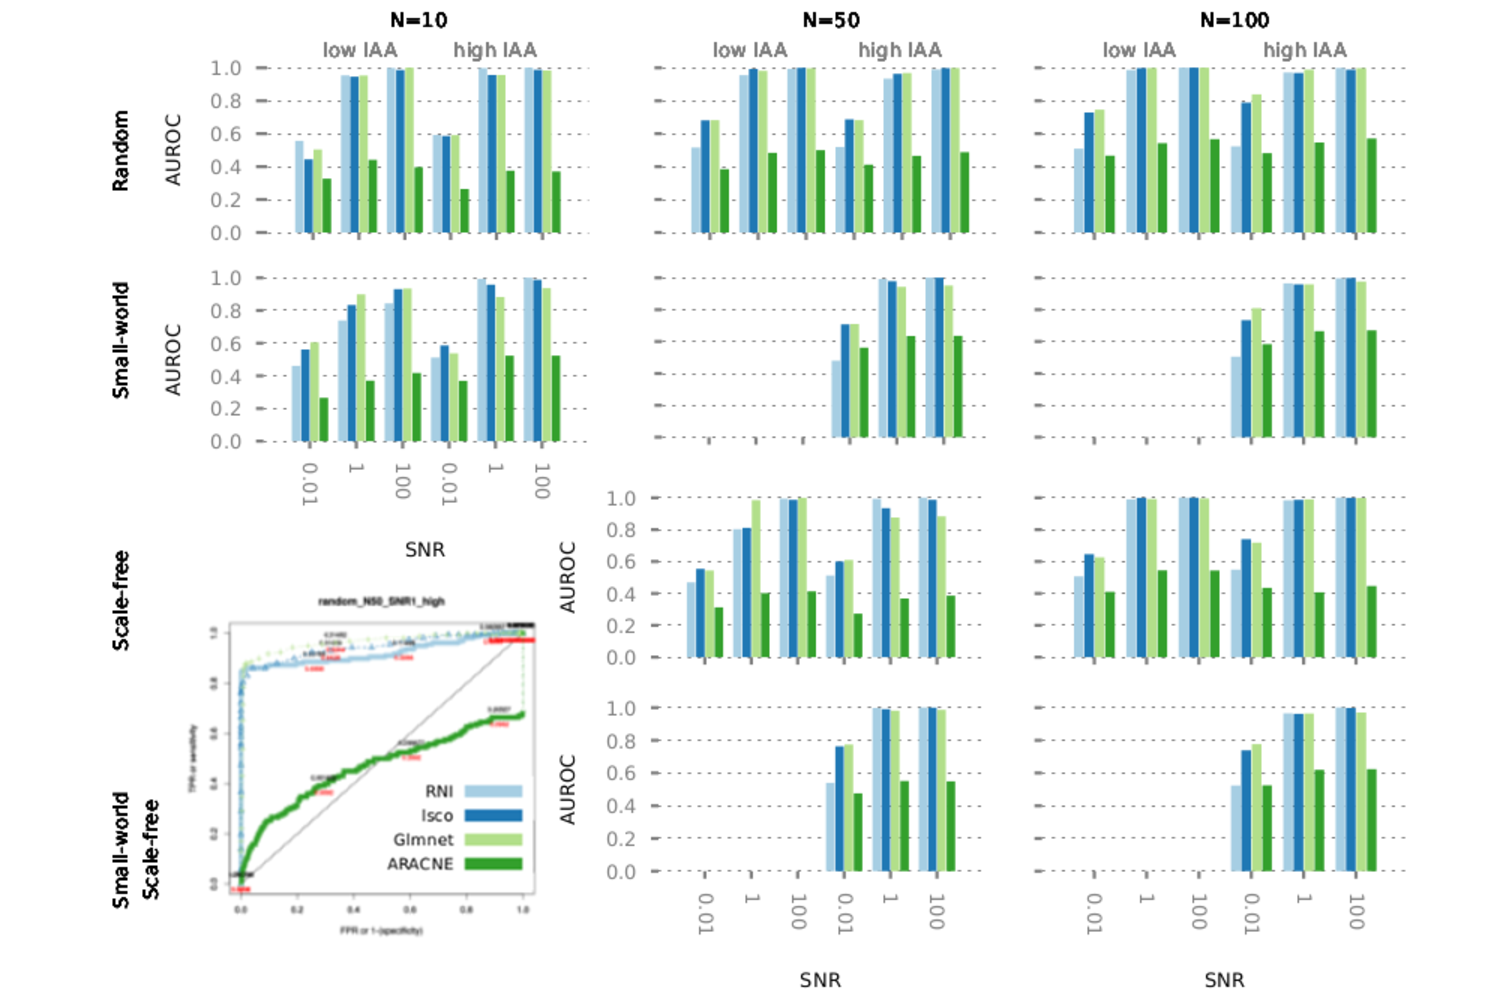
\includegraphics[width=.65\linewidth]{data_performance_early120916_POSTER.pdf}
% \end{center}
% }

%----------------------------------------------------------------------------------------
%	BOOTSTRAP PERFORMANCE
%----------------------------------------------------------------------------------------
\headerbox{Bootstrap Performance}{name=bootstrapPerf,span=2,column=1,below=workflow}{
\begin{minipage}[t]{0.33\textwidth}  \vspace{-3.75cm}
\begin{center}
% \vspace{.05cm}
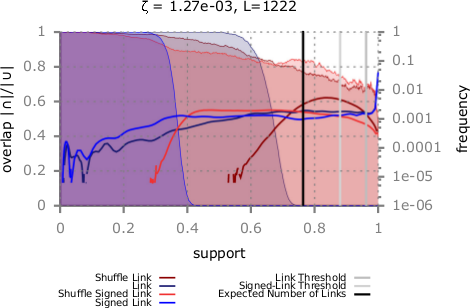
\includegraphics[width=1\linewidth]{1222.png}\\
\small \textit{\textbf{Figure 2.} Here we see a shuffled noise bubble in the middle of distinctive signaling links peaking on right edge. The frequency of bootstrap support for both shuffled and non shuffled data, existing and non-existing links.}
\end{center}
\end{minipage}
\begin{minipage}[t]{0.33\textwidth}  
\begin{center}
% \vspace{.05cm}
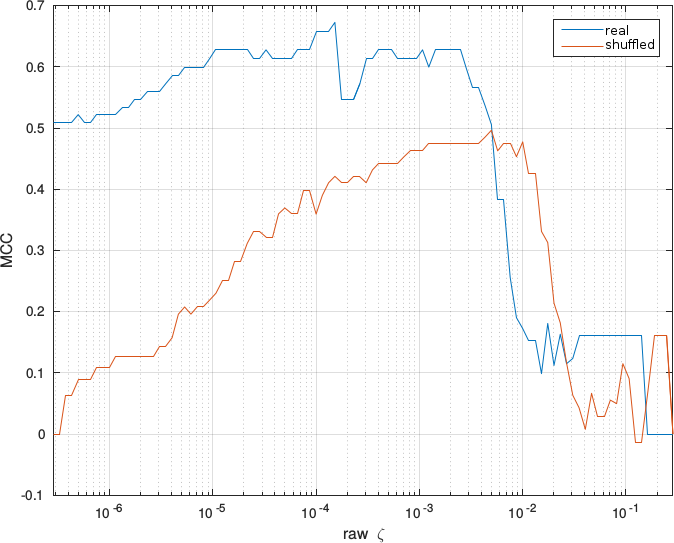
\includegraphics[width=1\linewidth]{MCC.png}\\
\small \textit{\textbf{Figure 3.} True link MCC is seen to outperform shuffled link until very dense networks. Performance in terms of MCC per sparsity.}
\end{center}
\end{minipage} 
\begin{minipage}[t]{0.33\textwidth} 
\begin{center}
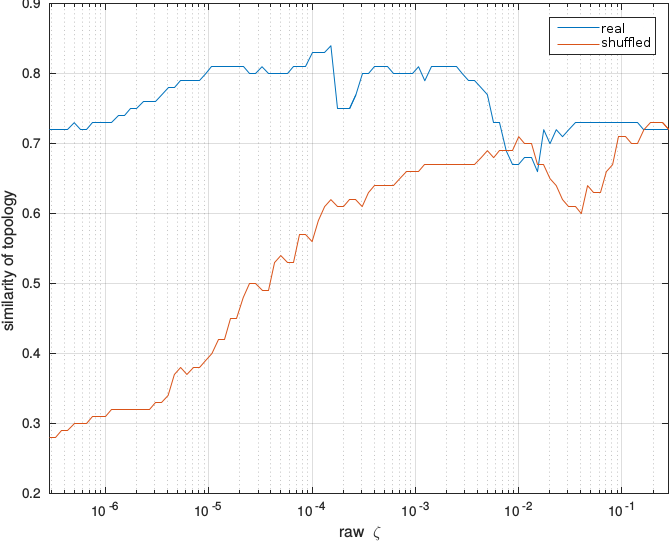
\includegraphics[width=1\linewidth]{ST.png}\\
\small \textit{\textbf{Figure 4.}True link Similarity of Topology (ST) is seen to outperform shuffled link until sufficiently dense networks. Performance in terms of ST per sparsity.}\\ 
% \vspace{0.05cm}
\end{center}
\end{minipage}  
}

%----------------------------------------------------------------------------------------
%	RESULTS
%----------------------------------------------------------------------------------------\headerbox{Introduction}{name=introduction,column=0,row=0, span=3}{

\headerbox{Conclusion}
{name=results,column=0,span=3,below=bootstrapPerf}{ %\hspace{0.1cm}
\begin{minipage}[t]{0.8\textwidth}  
\vspace{-3cm} 
We have developed a bootstrap-based method for estimating the accuracy of network inference through the use of L1-regularization methods. Benchmarking was enabled by simulated as well as  biological datasets. We also validate the inferred network by its ability to predict the effect of independent perturbations. Our shuffling paradigm restricted links to being novel, bidirectionally proportional, having equal self links as well as data properties, ie intrampatness (IAA). The goal is not simply to model, but to provide support for how realistic the presence of each link is, a key feature currently lacking in GRNI, in order to give practically useful insights into gene regulatory mechanisms.
As an example, we have included the MYC network, inferred with individual signed link confidence of over 95\% from a dataset consisting of 40 genes perturbed singly and doubly, and an average of all 100,000 bootstraps, 100 runs of 1000 bootstraps used to calculate the overlap as an indicator of stability. Using the nested bootstrap paradigm, we were able to infer the sign and direction of each link, with support for each exceeding 95\%.
% * <tn@kth.se> 2016-09-17T16:03:32.037Z:
%
% > We have developed a bootstrap-based method for estimating the accuracy of network inference through the use of L1-regularization methods. Benchmarking was enabled by simulated as well as  biological datasets. We also validate the inferred network by its ability to predict the effect of independent perturbations. The goal is not simply to model, but to provide support for how realistic the presence of each link is, a key feature currently lacking in GRNI, in order to give practically useful insights into gene regulatory mechanisms. 
%
% This is a good conclusion. If you want to have it as results please add some comment about the MYC network.
%
% ^.
%   \vspace{-0.25cm}
%   \end{center}
  \end{minipage}%\hfill
  \hspace{.75cm} %
\begin{minipage}[t]{0.15\textwidth}
% \begin{center}
\hspace{.5cm}
 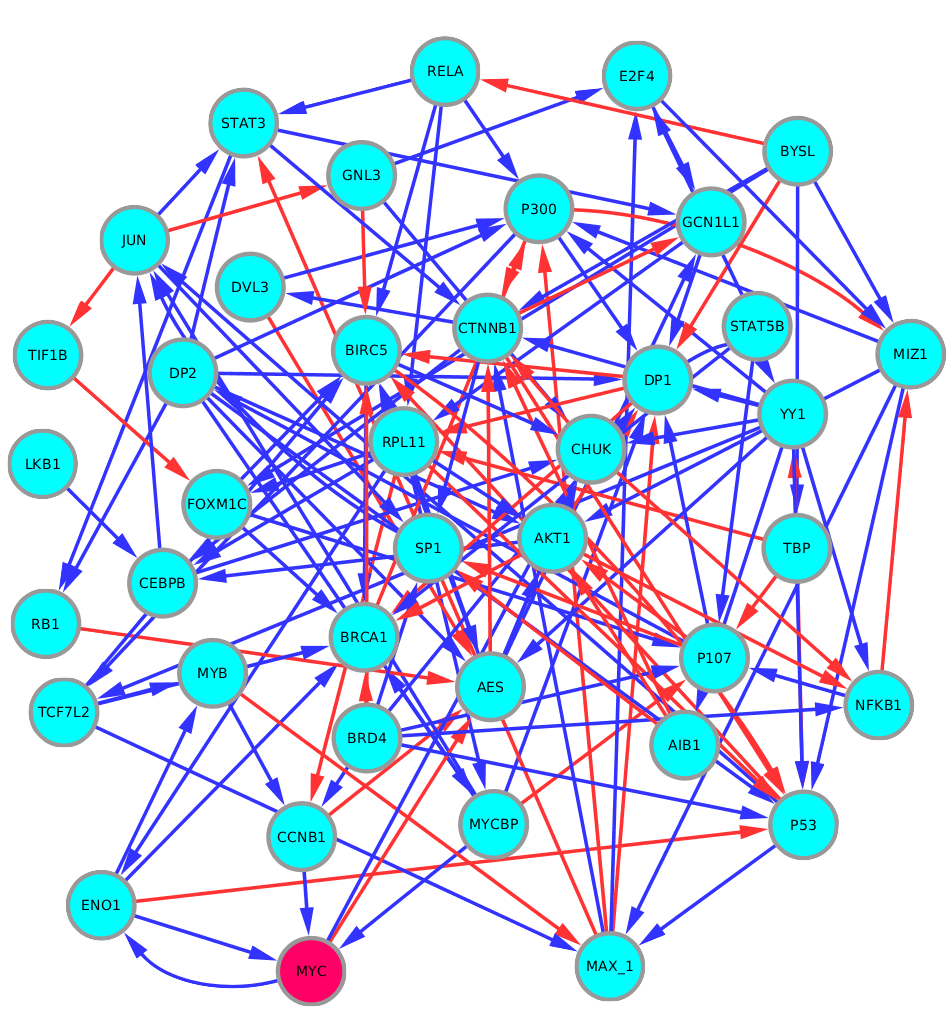
\includegraphics[width=.8\textwidth]{1031_c.png}\\ \small \textit{\textbf{Figure 5.} MYC signed link network}
% \end{center}
\end{minipage}
  
% * <tn@kth.se> 2016-09-17T16:05:37.453Z:
%
% > Example resultant
%
% This is the MYC network that you inferred, isn't it? Please say so instead of the cryptic example caption.
%
% ^.

% \vspace{0.2cm}

%  \centering\raisebox{\dimexpr 0.3\baselineskip-\height}{%
% 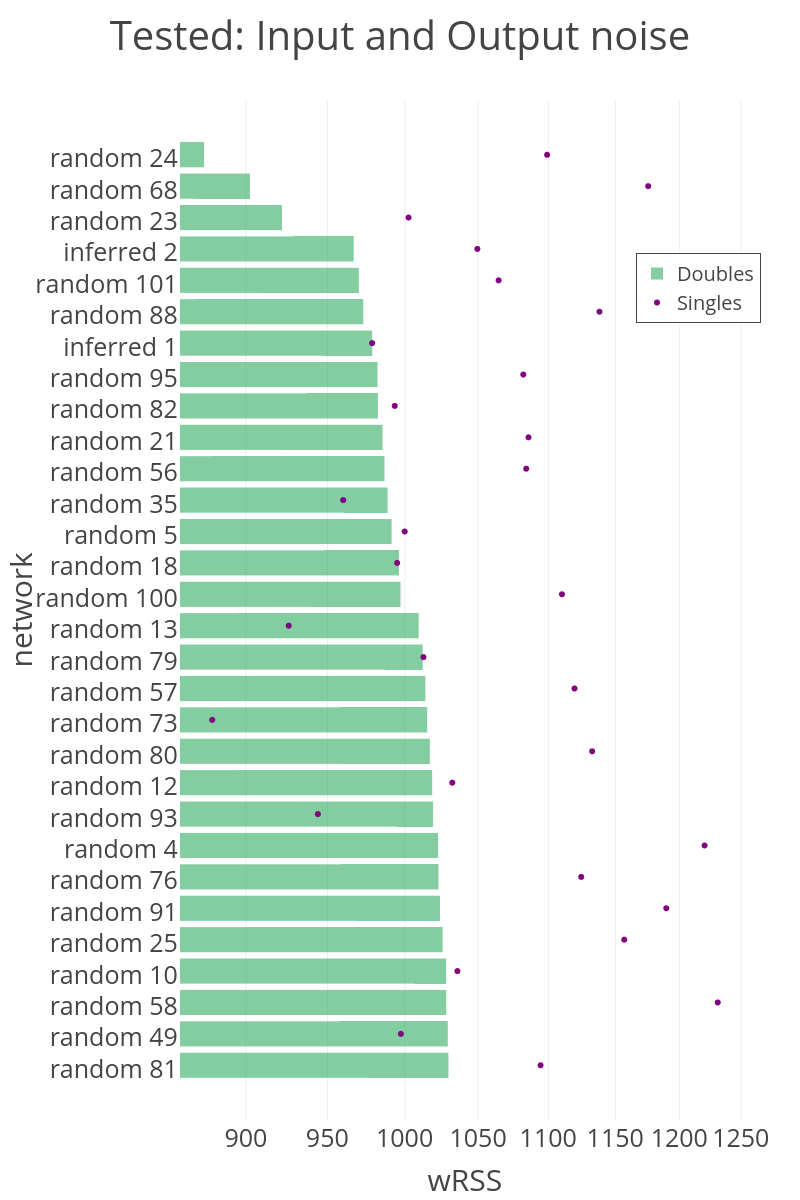
\includegraphics[width=.9\textwidth]{Tested__Input_and_Output_noise.png}
}
% %   \captionof{figure}{Caption for fig 1}



% 
% & \\
% %----------------------------------------------------------------------------------------
% %	CONCLUSION
% %----------------------------------------------------------------------------------------
% \headerbox{Conclusion}{name=conclusion,column=1,below=bootstrapPerf,span=2}{
% \vspace{-0.2cm}
% \begin{itemize} 
% \item We reveal highly observed, relevant interactions for inclusion in the model as well as a wash of random irrelevant interactions to disregard;
% \vspace{-0.2cm}
% \item LASSO and LSCO performed well when compared to randomly shuffled data (not shown);
% \vspace{-0.2cm}
% \item TLSCO has not yet been benchmarked and thus interpreting remains difficult;
% \vspace{-0.2cm}
% \item FUTURE DIRECTION:Repeat on datasets with controlled SNR, condition number and intrampatness including one test against high, medium and low of each, as well as datasets of established networks;
% \end{itemize}
% }


%----------------------------------------------------------------------------------------
%	REFERENCES
%----------------------------------------------------------------------------------------
\headerbox{References}{name=references,column=0,below=results, above=bottom,span=3}{
\smaller % Reduce the font size in this block
\renewcommand{\section}[2]{\vskip 0.05em} % Get rid of the default "References" section title
\nocite{Tjarnberg2014} % Insert publications even if they are not cited in the poster
\bibliographystyle{unsrt}
\bibliographystyle{IEEEtran}
\bibliography{biblio} % Use biblio.bib as the bibliography file
}
\end{poster}
\end{document}